% Options for packages loaded elsewhere
\PassOptionsToPackage{unicode}{hyperref}
\PassOptionsToPackage{hyphens}{url}
%
\documentclass[
]{article}
\usepackage{amsmath,amssymb}
\usepackage{lmodern}
\usepackage{iftex}
\ifPDFTeX
  \usepackage[T1]{fontenc}
  \usepackage[utf8]{inputenc}
  \usepackage{textcomp} % provide euro and other symbols
\else % if luatex or xetex
  \usepackage{unicode-math}
  \defaultfontfeatures{Scale=MatchLowercase}
  \defaultfontfeatures[\rmfamily]{Ligatures=TeX,Scale=1}
\fi
% Use upquote if available, for straight quotes in verbatim environments
\IfFileExists{upquote.sty}{\usepackage{upquote}}{}
\IfFileExists{microtype.sty}{% use microtype if available
  \usepackage[]{microtype}
  \UseMicrotypeSet[protrusion]{basicmath} % disable protrusion for tt fonts
}{}
\makeatletter
\@ifundefined{KOMAClassName}{% if non-KOMA class
  \IfFileExists{parskip.sty}{%
    \usepackage{parskip}
  }{% else
    \setlength{\parindent}{0pt}
    \setlength{\parskip}{6pt plus 2pt minus 1pt}}
}{% if KOMA class
  \KOMAoptions{parskip=half}}
\makeatother
\usepackage{xcolor}
\usepackage{longtable,booktabs,array}
\usepackage{calc} % for calculating minipage widths
% Correct order of tables after \paragraph or \subparagraph
\usepackage{etoolbox}
\makeatletter
\patchcmd\longtable{\par}{\if@noskipsec\mbox{}\fi\par}{}{}
\makeatother
% Allow footnotes in longtable head/foot
\IfFileExists{footnotehyper.sty}{\usepackage{footnotehyper}}{\usepackage{footnote}}
\makesavenoteenv{longtable}
\usepackage{graphicx}
\makeatletter
\def\maxwidth{\ifdim\Gin@nat@width>\linewidth\linewidth\else\Gin@nat@width\fi}
\def\maxheight{\ifdim\Gin@nat@height>\textheight\textheight\else\Gin@nat@height\fi}
\makeatother
% Scale images if necessary, so that they will not overflow the page
% margins by default, and it is still possible to overwrite the defaults
% using explicit options in \includegraphics[width, height, ...]{}
\setkeys{Gin}{width=\maxwidth,height=\maxheight,keepaspectratio}
% Set default figure placement to htbp
\makeatletter
\def\fps@figure{htbp}
\makeatother
\setlength{\emergencystretch}{3em} % prevent overfull lines
\providecommand{\tightlist}{%
  \setlength{\itemsep}{0pt}\setlength{\parskip}{0pt}}
\setcounter{secnumdepth}{-\maxdimen} % remove section numbering
\ifLuaTeX
  \usepackage{selnolig}  % disable illegal ligatures
\fi
\IfFileExists{bookmark.sty}{\usepackage{bookmark}}{\usepackage{hyperref}}
\IfFileExists{xurl.sty}{\usepackage{xurl}}{} % add URL line breaks if available
\urlstyle{same} % disable monospaced font for URLs
\hypersetup{
  pdftitle={Deshacer su casa interior es difícil},
  hidelinks,
  pdfcreator={LaTeX via pandoc}}

\title{Deshacer su casa interior es difícil}
\author{}
\date{}

\begin{document}
\maketitle

\subsection{Breaking Up Is Hard to Do}

Traducción aproximada del Artículo de \textbf{Kit Woolsey}, publicado en
\emph{Backgammon Galore} :
\url{https://bkgm.com/articles/GOL/Nov99/break.htm}

\begin{figure}
\centering
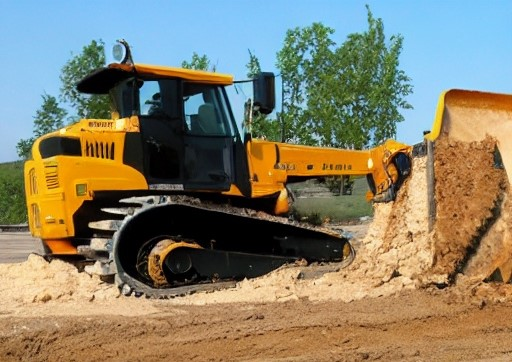
\includegraphics{/images/cad-driving-bulldozer.jpg}
\caption{Demoliendo Casa}
\end{figure}

La primera vez que revisé partidas jugadas por \emph{TD-Gammon} (el
primer programa de juego de Backgammon de red neuronal), busqué jugadas
inusuales que fueran diferentes de lo que yo hubiera hecho. Un tema
recurrente que noté fue que \emph{TD-Gammon} a menudo en un juego de
espera (\emph{holding game}) deshacía su casa interior, sin razón
aparente. Por ejemplo:

\begin{figure}
\centering
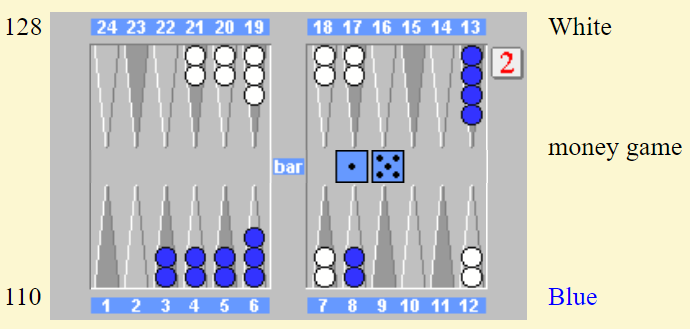
\includegraphics{/images/VsHG-Diagrama-01.png}
\caption{Diagrama 01}
\end{figure}

¿Qué podría ser más obvio que \textbf{13/8, 6/5}, verdad? ¡Sin embargo,
\emph{TD-Gammon} jugó el aparentemente inexplicable \textbf{13/8, 3/2} !
Inicialmente supuse que era una de esas peculiaridades de los programas
de redes neuronales. Sabía que en posiciones simples los programas a
menudo hacen movimientos extraños (y equivocados) porque su
entrenamiento no les da suficiente información para trabajar con los
principios correctos. Los expertos humanos generalmente superarán a los
\emph{bots} en este tipo de posiciones cuando se trata de pequeñas
diferencias técnicas. Bromeé sobre esto con Gerry Tesauro, el inventor
de \emph{TD-Gammon}, y lo llamé el \emph{juego extraño de TD}.

Un poco más tarde, cuando Gerry había programado \emph{TD-Gammon} para
analizar posiciones, le pedí que analizará un par de estos tipos de
jugadas, solo para estar seguro. Para mi sorpresa, las \emph{jugadas
extrañas de TD} superaron consistentemente a las jugadas normales en el
análisis. Esto era otra cosa. Si bien el programa podría tener algunas
ideas extrañas, generalmente funcionó bien y era difícil ver cómo podría
arruinar los análisis para una posición como esta. Incluso si hubiera
algún tipo de sesgo en los juegos de retención del programa, las
posiciones después de las dos jugadas en cuestión son tan similares que
el sesgo ciertamente se aplicaría a cualquiera de los dos juegos, por lo
que los resultados del análisis serían precisos. El valor absoluto puede
no ser correcto, si el \emph{bot} está jugando mal en un lado o en el
otro, pero los resultados relativos entre las dos jugadas casi tienen
que ser precisos.

De improviso, no parece que pueda haber mucha diferencia, incluso si una
jugada fuera superior. Los análisis muestran que la diferencia puede ser
más significativa de lo que pensamos. Hice que \emph{Snowie} hiciera
rodar las dos jugadas (1-ply, sin cubo, 3888 veces cada una con los
mismos dados) y los resultados fueron:

\begin{longtable}[]{@{}lll@{}}
\toprule()
Jugada & ~\textbackslash{} & Equidad \\
\midrule()
\endhead
\textbf{13/8, 3/2} & & \textbf{+0.410} \\
\textbf{13/8, 6/5} & & +0.362 \\
\bottomrule()
\end{longtable}

Es una diferencia bastante significativa para lo que parece ser un
\textbf{\emph{1}} casi sin sentido. De acuerdo, el tamaño de la muestra
no es enorme, pero con los dados duplicados y la similitud de las
posiciones, parece bastante claro que el \emph{juego extraño de TD} es
notablemente superior. Este no es un caso aislado. Encontré que este
tipo de juego ganó consistentemente en los análisis. ¿Qué está pasando?

Miremos hacia adelante y veamos cómo es probable que continúe el juego.
Está claro que el Azul no va a ser capturado durante bastante tiempo. El
Blanco está atrasado en la carrera, por lo que incluso si tuviera una
tirada gratis para despejar el punto de barra, preferiría permanecer
allí para mantener el contacto. Solo si el Blanco sacará un doble
elevado, consideraría dejar el ancla. Por lo tanto, no hay una necesidad
urgente de cerrar los puntos internos del tablero para las próximas
tiradas.

Si el Azul lanza dobles, por supuesto despejará el punto medio y
probablemente ganará la carrera. No importará mucho qué \emph{1} haya
jugado; pero separarse a la casilla 2 diversifica las fichas del Azul
para la extracción (Bear-off), por lo que no puede ser malo. De manera
similar, si el Blanco obtiene dobles grandes, podrá correr con el ancla
y convertir el juego en una carrera pura. Una vez más, separarse a la
casilla 2 está bien. El escenario más interesante ocurre cuando ninguno
obtiene dobles durante varias tiradas. El Azul tendrá que traer sus
fichas lo mejor que pueda. Su primera prioridad será jugar seguro, pero
también quiere desperdiciar lo menos posible. Un gran doble del Blanco
convertirá el juego en una carrera pura, y si el Azul ha desperdiciado
demasiado, su ventaja en pips se irá por el desagüe. El objetivo del
Azul es completar su casa interior sin problemas, evitando huecos en las
casillas inferiores. Esto será lo mejor tanto para la carrera; como si
el Blanco deshace el ancla y captura una ficha del Azul. Lo que el Azul
quiere evitar es apilar un montón de fichas en una casilla y dejar otra
vacía.

Ahora que vemos lo que el Azul está tratando de lograr, queda más claro
por qué \textbf{13/8, 3/2} es superior a \textbf{13/8, 6/5}. En primer
lugar, tener el repuesto en la casilla 6 es definitivamente una ventaja,
ya que aumenta la flexibilidad del Azul. Más importante aún, la
separación a la casilla 2 mejora las posibilidades del Azul de aplanar
la posición. Después de la división, si una ficha Azul cae en la casilla
3 o en la 2, se ve bien. Si el Azul juega \textbf{13/8, 6/5}, entonces
necesita que una ficha caiga precisamente en la casilla 2 para que
funcione el proceso de aplanado.

Como ilustración, supongamos que el Blanco obtiene \textbf{\emph{6-4}}
jugando \textbf{13/7, 13/9} y la siguiente tirada del Azul es
\textbf{\emph{6-4}}. Naturalmente el Azul traerá una ficha desde el
punto medio. El Azul quiere despejar el punto medio lo antes posible, y
quiere mantener repuestos en la casilla 8 para manejar dados difíciles.
Si el Azul hubiera jugado \textbf{13/8, 6/5}, la posición después de que
juegue ahora \textbf{13/3} se vería así:

\begin{figure}
\centering
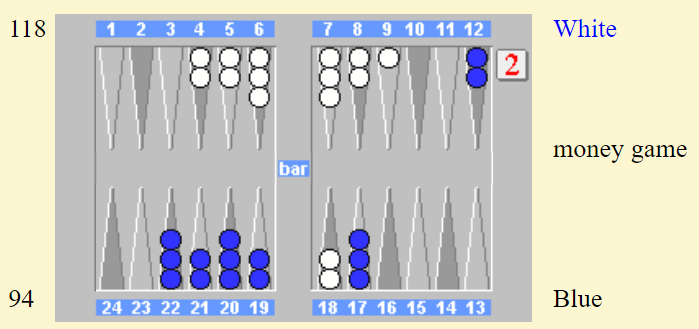
\includegraphics{/images/VsHG_Diagrama_02.png}
\caption{Diagrama 02}
\end{figure}

Empieza a verse un poco feo. Tres fichas en la casilla 3 y las casilla 1
y 2 aún vacías. Esa tercera ficha en la casilla 3 pertenece a la 2, pero
no llegará allí a menos que el Azul saque un \textbf{\emph{1}}. La clave
es que el Azul sacó ese \textbf{\emph{1}} en su turno anterior, y ahí es
cuando la ficha debería haberse movido a la casilla 2. Si el Azul
hubiera jugado correctamente, la posición se vería así:

\begin{figure}
\centering
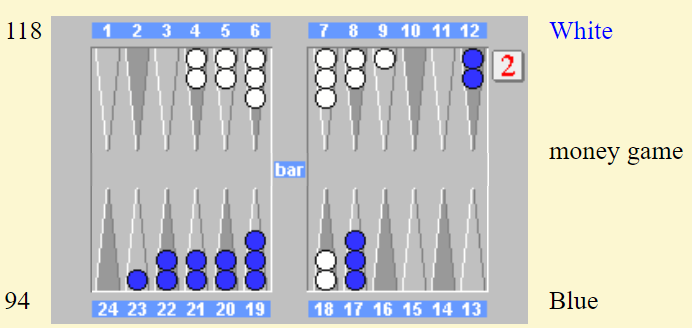
\includegraphics{/images/VsHG_Diagrama_03.png}
\caption{Diagrama 03}
\end{figure}

¿No es mucho más agradable? Ahora bien, si la siguiente tirada del Azul
es algo así como \textbf{\emph{5-3}}, puede jugarlo decentemente sin
enredarse. En la posición con tres fichas en la casilla 3 y la casilla 6
despojada, una tirada de \textbf{\emph{5-3}} se juega terriblemente.

Reconozco que elegí una secuencia de tiradas particularmente incómoda
para que el Azul ilustrara mi punto. Sin embargo, estas secuencias
incómodas son las que importan. Si el Azul saca un montón de
\textbf{\emph{2-1}}, no habrá ninguna diferencia en cómo jugó las
tiradas anteriores, ya que tendrá la oportunidad de volver a colocar sus
fichas donde pertenecen. Son los dados grandes, como
\textbf{\emph{6-4}}, los que crean la incomodidad si no ha planificado
con anticipación y colocado sus fichas correctamente.

\begin{figure}
\centering
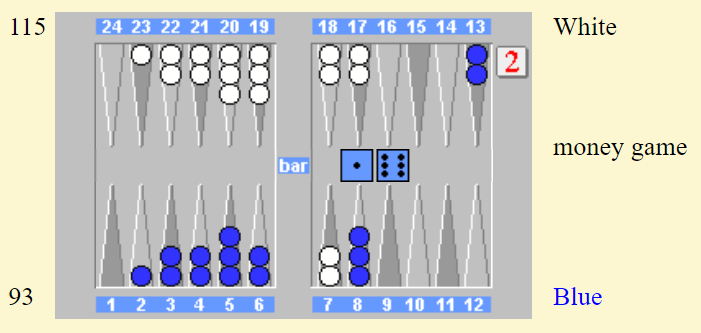
\includegraphics{/images/VsHG_Diagrama_04.png}
\caption{Diagrama 04}
\end{figure}

El Azul debería jugar \textbf{8/1}, no \textbf{8/2 5/4}. Esta es una
jugada bastante importante. El problema es que si el Azul saca un
\textbf{\emph{6}} a continuación, tendrá que despejar su casilla 8 para
jugar seguro. Si el Azul ha jugado \textbf{8/2, 5/4}, entonces este
\textbf{\emph{6}} lo obligará a poner una tercera ficha en la casilla 2,
lo cual es horrible por consideraciones de flexibilidad, carrera y
construcción del tablero. Después de jugar \textbf{8/1}, el Azul pondrá
una segunda ficha en la casilla 2, lo cual está bien.

Lo principal que debe tener en cuenta al considerar este tipo de juego,
que deshace su casa interior, es que no será capturado en los próximos
dos turnos, por lo que tendrá tiempo para volver a construir su casa. Si
está adelantado en la carrera, este es casi siempre el caso; ya que su
oponente se quedará atrás para mantener el mayor contacto posible. Sin
embargo, si está atrasado en la carrera, deshacer su casa puede darle a
su oponente la oportunidad de \emph{pagar ahora y correr}. Por ejemplo:

\begin{figure}
\centering
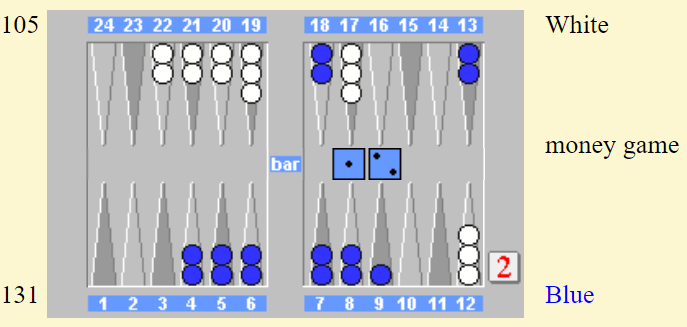
\includegraphics{/images/VsHG_Diagrama_05.png}
\caption{Diagrama 05}
\end{figure}

Dado que el Blanco tiene tres fichas en el punto medio, no hay forma de
el Azul pueda capturar en la tirada siguiente. Incluso si el Azul
deshace su casa, el Blanco no moverá dos fichas desde el punto medio, ni
dejará fichas vulnerables. Por lo tanto, el Azul puede y debe jugar
\textbf{8/6, 4/3}. Esto le facilitará apoderarse de las casillas 4 y 3
en sus próximas tiradas, que es lo que está tratando de conseguir. Hay
poco peligro en deshacer temporalmente la casilla 4, ya que el Azul
tiene varias tiradas para rehacerlo. Si el Azul en cambio juega
\textbf{9/6}, tendrá obtener dados perfectos para lograr la casilla 3.
Para ver la diferencia, imagine que en la siguiente tirada el Azul lanza
\textbf{\emph{6-1}} y observe cómo jugar los dados ambas posiciones.

Una pequeña modificación de la posición puede cambiar las cosas.
Considere la siguiente:

\begin{figure}
\centering
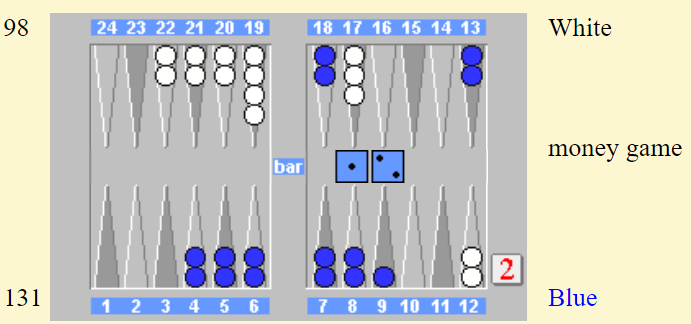
\includegraphics{/images/VsHG_Diagrama_06.png}
\caption{Diagrama 06}
\end{figure}

La misma posición excepto que ahora el Blanco solo tiene dos fichas en
su punto medio. La diferencia es que el Azul podría capturar en la
siguiente tirada. Si el Blanco lanza algo como \textbf{\emph{5-3}},
puede optar por \emph{pagar ahora} y jugar \textbf{13/8, 13/10}. Este
pago es obviamente más atractivo si la casa del Azul es un desastre. Por
lo tanto, el Azul debería jugar el normal \textbf{9/6} en lugar del
excéntrico juego de deshacer su casa.

La mayoría de los jugadores está familiarizada con las jugadas de
intercambio de casillas en situaciones de \emph{ataque} (blitz); en las
que cambia para obtener una casilla más baja, y para tener más
constructores apuntando a la casilla vulnerable. Si no puede mover los
constructores a la casilla, mueva la casilla hacia los constructores. El
mismo principio se puede aplicar en los juegos de retención, utilizando
jugadas que deshacen su casa.

\begin{figure}
\centering
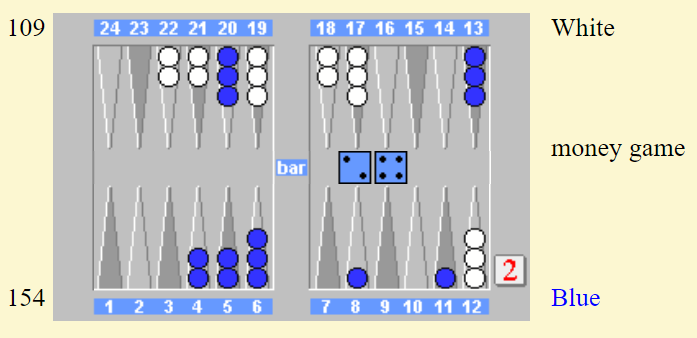
\includegraphics{/images/VsHG_Diagrama_07.png}
\caption{Diagrama 07}
\end{figure}

Creo que la mejor jugada del Azul es la extraña \textbf{13/9, 5/3}. El
Blanco definitivamente no dejará una vulnerabilidad en la próxima
tirada, por lo que el Azul puede permitirse deshacer su casa
temporalmente. La pérdida de la casilla 5 no es significativa, ya que el
Azul la recuperará con cualquier tirada excepto \textbf{\emph{5-2}}. La
clave es que el Azul se inserta en la casilla 3, que es la próxima que
quiere lograr. Si el Azul hace otra jugada, la casilla 3 permanecería
vacía; y generalmente el Azul podrá insertarse y conseguir la casilla 3,
antes de que el Blanco deje una ficha vulnerable, ocasionalmente los
dados pueden no cooperar. En esencia, la jugada \textbf{5/3} del Azul
activa el constructor de la casilla 11 sin tener que mover la ficha.
Naturalmente, si el Blanco tuviera solo dos fichas en el punto medio, el
Azul no podría permitirse el lujo de deshacer su casa, ya que el Blanco
podría ofrecer una ficha vulnerable y despejar su punto medio.

Por supuesto, las ganancias de estas jugadas que deshacen la casa
interior son pequeñas, pero todo ayuda. Nuestro objetivo es maximizar
nuestra equidad todo el tiempo. Además, este tipo de posición es muy
común, por lo que las ganancias acumuladas en muchos juegos pueden ser
significativas. La próxima vez que esté construyendo su casa interior,
mientras se enfrenta a un juego de retención, y parezca que sus jugadas
son incómodas, y está atado a un nudo; vuelva atrás y vea si perdió la
oportunidad de una rentable jugada para deshacer su casa. Es probable
que descubra que esos dados incómodos se habrían jugado mucho mejor si
se hubiera preparado adecuadamente.

\end{document}
